\documentclass[11pt,letterpaper]{article}

\usepackage{setspace}
%\doublespacing
\linespread{1.25}
%\linespread{2}
\usepackage{geometry}

\geometry{letterpaper, margin=1in}
%\usepackage{times}
\usepackage{pslatex}
\usepackage{apacite}
\usepackage{url}
\usepackage{graphicx}
\usepackage{caption}
\usepackage{subcaption}
\usepackage{listings}
\usepackage{color}
\usepackage{textcomp}
\usepackage{amsmath}
\usepackage{amssymb}
\usepackage{wrapfig}
\usepackage{lipsum}

\graphicspath{{figures/}}

\def\signed #1{{\leavevmode\unskip\nobreak\hfil\penalty50\hskip2em
  \hbox{}\nobreak\hfil(#1)%
  \parfillskip=0pt \finalhyphendemerits=0 \endgraf}}

\newsavebox\mybox
\newenvironment{aquote}[1]
  {\savebox\mybox{#1}\begin{quote}}
  {\signed{\usebox\mybox}\end{quote}}


 \newcommand{\denote}[1]{\mbox{ $[\![ #1 ]\!]$}}

\definecolor{Red}{RGB}{255,0,0}
\newcommand{\red}[1]{\textcolor{Red}{#1}}  
\definecolor{Green}{RGB}{10,200,100}
\definecolor{Blue}{RGB}{10,100,200}
\newcommand{\ndg}[1]{\textcolor{Green}{[ndg: #1]}}  
\newcommand{\mht}[1]{\textcolor{Blue}{[mht: #1]}}  

\usepackage{titlesec}

\setcounter{secnumdepth}{4}

\titleformat{\paragraph}
{\normalfont\normalsize\bfseries}{\theparagraph}{1em}{}
\titlespacing*{\paragraph}
{0pt}{3.25ex plus 1ex minus .2ex}{1.5ex plus .2ex}

\title{Talking in generalizations}
\author{{\large \bf Michael Henry Tessler} and {\large \bf Noah D. Goodman} \\
\{mtessler, ngoodman\} @stanford.edu\\
  Department of Psychology, Stanford University}

\begin{document}

\maketitle

Learning and development require solving problems of induction.
These are hard problems though they can be solved by adults and young children with observational learning \cite{Markman1989} 
and in pedagogically enriched scenarios \emph{(CITE SOME PEDAGOGY}).
At about age of the two, a new tool for communication and learning is available: language.

Generalizations are central to human understanding and thus, it is not surprising that language provides a simple and ubiquitous way to communicate these generalizations. 
Generic language (e.g.~\emph{Swans are white.}) convey generalizations about categories \cite{Carlson1977, Leslie2008}. 
Generics are ubiquitous in everyday conversation as well as in child-directed speech \cite{Gelman2008}, and children as young as two or three understand that generics refer to categories and support generalization \cite{Cimpian2008}.
They are thought to be essential to the growth of conceptual knowledge \cite{Gelman2004} and how kinds are represented in the mind \cite{Leslie2008}, and yet a formal account of generic meaning remains elusive. 

The primary hurdle in formalizing generic language ) is in determine what makes a generic sentence true or false (i.e. the truth conditions).
Generics look a lot like quantifier statements (e.g. \emph{some, all, most}).
At first blush, they look like universally quantified statements as in \emph{All swans are white}, and yet generics---unlike universals---admit exceptions (e.g. there are black swans). 
Interpreting the generic as meaning ``most'' (i.e. \emph{Most swans are white}) captures many cases but fails to account for others: \emph{Robins lay eggs} seems true even though only adult, female robins do; only a tiny fraction of Mosquitos carry the virus Zika yet \emph{Mosquitos carry Zika} also sounds true. 
In fact, the very notion that the felicity of the generic can be tied to how many instances have the property (in the way that quantifier statements are) violates intuitions: \emph{Robins lay eggs} even though only the females do but \emph{Robins are female} (even though only the females are) is not a reasonable utterance.

%Habitual sentences behave in an analogous way. 
%Bill may smoke a pack a day and so we would say \emph{Bill smokes}, and if Bill goes without a cigarette for an entire family vacation (thus temporarily reducing his effective rate of smoking), we will not be so easily convinced (i.e. \emph{Bill smokes} is probably still true).
%Cases like \emph{Mosquitos carry malaria} (wherein only a tiny percentage have the property) seem to parallel habitual sentences of rare actions like \emph{Susan writes novels}. Susan may only have written 3 novels in her life, but still this seems like a valid generalization to convey.

We argue that the core meaning of a generic sentence is simple but underspecified, and that general principles of pragmatic reasoning are responsible for establishing a precise meaning in context. 
Building on recent probabilistic models of language understanding, we provide a formal model for the evaluation of generic sentences. 
This model explains the puzzling flexibility in truth conditions in terms of diverse prior beliefs about properties.
In Experiment 1, we elicit these priors experimentally and show that the resulting model predictions explain almost all of the variance in human judgments for both common generic sentences.
Experiment 2 provides a conceptual replication using habitual sentences (e.g. \emph{Bill smokes}) that describe generalizations about events (e.g. \emph{smoking a cigarette}; \citeNP{Carlson1977, Carlson2005, Cohen1999}).
%In Experiment 3, we show that habituals are sensitive to top-down moderators of expected frequency: It is the expectation of future tendency that matters for habitual language.

\subsubsection*{A formal model of generic meaning}

Generics express a relation between a kind (e.g. \textsc{robins}) and a property (e.g. \textsc{lays eggs}). 
For a given kind $K$ (e.g.~\textsc{robins}) and property $F$ (e.g.~\textsc{lays eggs}), we refer to the probability that an object of kind $K$ has property $F$, that is $P(F\mid K)$, as the \emph{prevalence} of $F$ within $K$.\footnote{Because we aim to explain the psycholinguistics of generics, we are generally interested in the subjective probability, not the actual frequency in the world.}
Logical quantifiers can be described as conditions on prevalence (i.e.~\emph{some} is $P(F\mid K)>0$, \emph{all} is $P(F\mid K)=1$). 
Extending this, it seems the simplest meaning for generic statements would be a similar threshold on prevalence: $P(F\mid K)>\tau$ \cite{Cohen1999}. 
However, no fixed value of the threshold, $\tau$, would allow for the extreme flexibility generics exhibit (e.g. \emph{Robins lay eggs} vs. \emph{Robins are female}; \emph{Mosquitos carry malaria}).
Building on \citeA{Lassiter2013,Lassiter2015}, we posit that this threshold is not a fixed property of the language, but is established by pragmatic inference.

Using the Rational Speech-Acts framework \cite{Frank2012,Goodman2013}, 
we model a speaker $S_2$ who reasons about a pragmatic listener $L_1$; this listener is considering the propensity of a certain behavior of an individual.
The listener $L_1$ has uncertainty about the appropriate threshold for the habitual in this context ($\tau \sim \text{Uniform}$(0,1)), and reasons about what an informative speaker $S_1$ would be likely to say. The hypothetical speaker $S_1$ in turn reasons about an idealized literal listener $L_0$, who has access to the threshold $\tau$ (i.e. $S_1$ believes $L_0$ will interpret him in exactly the way he means). 
Writing the prevalence as $x$, this leads to a set of equations:
\begin{eqnarray}
P_{S_{2}}(u \mid x) & \propto &  \int_{\tau} P_{L_{1}}(x , \tau \mid u) \label{eq:S2}\\
P_{L_{1}}(x , \tau \mid u) &\propto& P_{S_{1}}(u \mid x, \tau) \cdot P(x) \cdot P(\tau) \label{eq:L1}\\
P_{S_{1}}(u \mid x, \tau) &\propto&  {P_{L_{0}}(x \mid u, \tau)}^{\alpha} \label{eq:S1}\\
P_{L_{0}}(x \mid u, \tau) &\propto& {\delta_{\denote{u}(x, \tau)} P(x)}. \label{eq:L0}
\end{eqnarray}
We take the pragmatic speaker $S_2$ to consider two utterances: the generic, with $\denote{u}(x, \tau) := x>\tau$, or nothing (staying silent), with $\denote{u}(x, \tau) := \text{True}$.
Equation \ref{eq:S2} can then be interpreted as a model of felicity or truth judgments \cite{Degen2014, TesslerUnderReview}.
The speaker will choose to produce the habitual when the true prevalence $x$ is more likely under $L_1$'s posterior given the generic than under her prior (implied by $S_2$ ``staying silent''). 
A fully implemented version of the model can be found at \url{http://forestdb.org/models/generics.html}.

\subsubsection*{Summary of experiments}

The prior $P(x)$ (in Eqs.~\ref{eq:L1}, \ref{eq:L0}) describes the belief distribution on the prevalence of a given property (e.g. \textsc{lays eggs}) across relevant categories. 
%The shape of this distribution affects model predictions, but may vary significantly among different properties.
We measured it empirically (n=60) for a set of properties (e.g. \textsc{lays eggs, carries malaria}; 21 in total) used in our target sentences. 
 
%\subsubsection*{Method}
%
%We recruited 60 participants over Amazon's crowd-sourcing platform Mechanical Turk (MTurk).  
%%We chose this number of participants based on intuition with similar experiments and model comparison; 
%%since this is a quantitative experiment with no planned comparisons, power analysis in not appropriate.
%Participants were restricted to those with US IP addresses and with at least a 95\% MTurk work approval rating (the same criteria apply to all experiments reported). 
%
%On each trial of the experiment, participants filled out a table where each row was an animal category and each column was a property. 
%In order to alleviate the dependence of the distribution on our animal categories of interest, half of the animal categories were self-generated by the participant; the other half were randomly sampled from a set corresponding to the generic sentences used in Expt. 1b (e.g. \textsc{robins, mosquitos}).
%Participants were asked to fill in each row with the percentage of members of each of the species that had the property (e.g. ``50\%'').
%Each participant reported on sixteen properties (see {\it SI Section A} for more details).
%We used a set of properties associated with generics of theoretical interest (twenty-one properties in total), as described above.
% 
%\subsubsection*{Data analysis and results}
 
While each $P(x)$ is a single distribution on prevalence, it may be structured as the result of deeper conceptual knowledge. 
For instance, if participants believe that some kinds have a causal mechanism that \emph{could} give rise to the property, while others do not, then we would expect $P(x)$ to be structured as a mixture distribution (cf. \citeA{Griffiths2005}).
If a kind can have the property, we assume the prevalence follows a Beta distribution with mean $\gamma$ and concentration $\xi$. 
If a kind cannot, the prevalence can only be 0\%.
The relative contribution of these two components is governed by mixture parameter $\theta$, inferred from the data.\footnote{This is similar in spirit to Hurdle Models of epidemiological data, where the observed count of zeros is often substantially greater than one would expect from standard models, such as the Poisson (e.g. adverse events to vaccines)\cite{hurdleModels}}
Thus, $\theta$ is the potential of a property to be present in a kind and $\gamma$ is the mean prevalence of the property among the kinds with the potential to have it (see Figure~\ref{fig:priors1} scatter). 
The prevalences given by participants would then be distributed as: $P(d) = \theta \cdot \text{Beta}(d \mid \gamma,\xi)+ (1 - \theta) \cdot \delta_{d=0} $. 
We put uninformative priors over all the parameters, $\theta \sim \text{Uniform}(0,1)$, 
$\gamma \sim \text{Uniform}(0,1)$, $\xi \sim \text{Uniform}(0, 50)$, and implemented this Bayesian statistical model using the probabilisitic programming language WebPPL \cite{dippl}. 
This statistical model reproduced the prior elicitation data with a low reconstruction error ($r^2 = 0.94$), strongly supporting the assumption of a structured prior. 


\begin{figure*}
\centering
    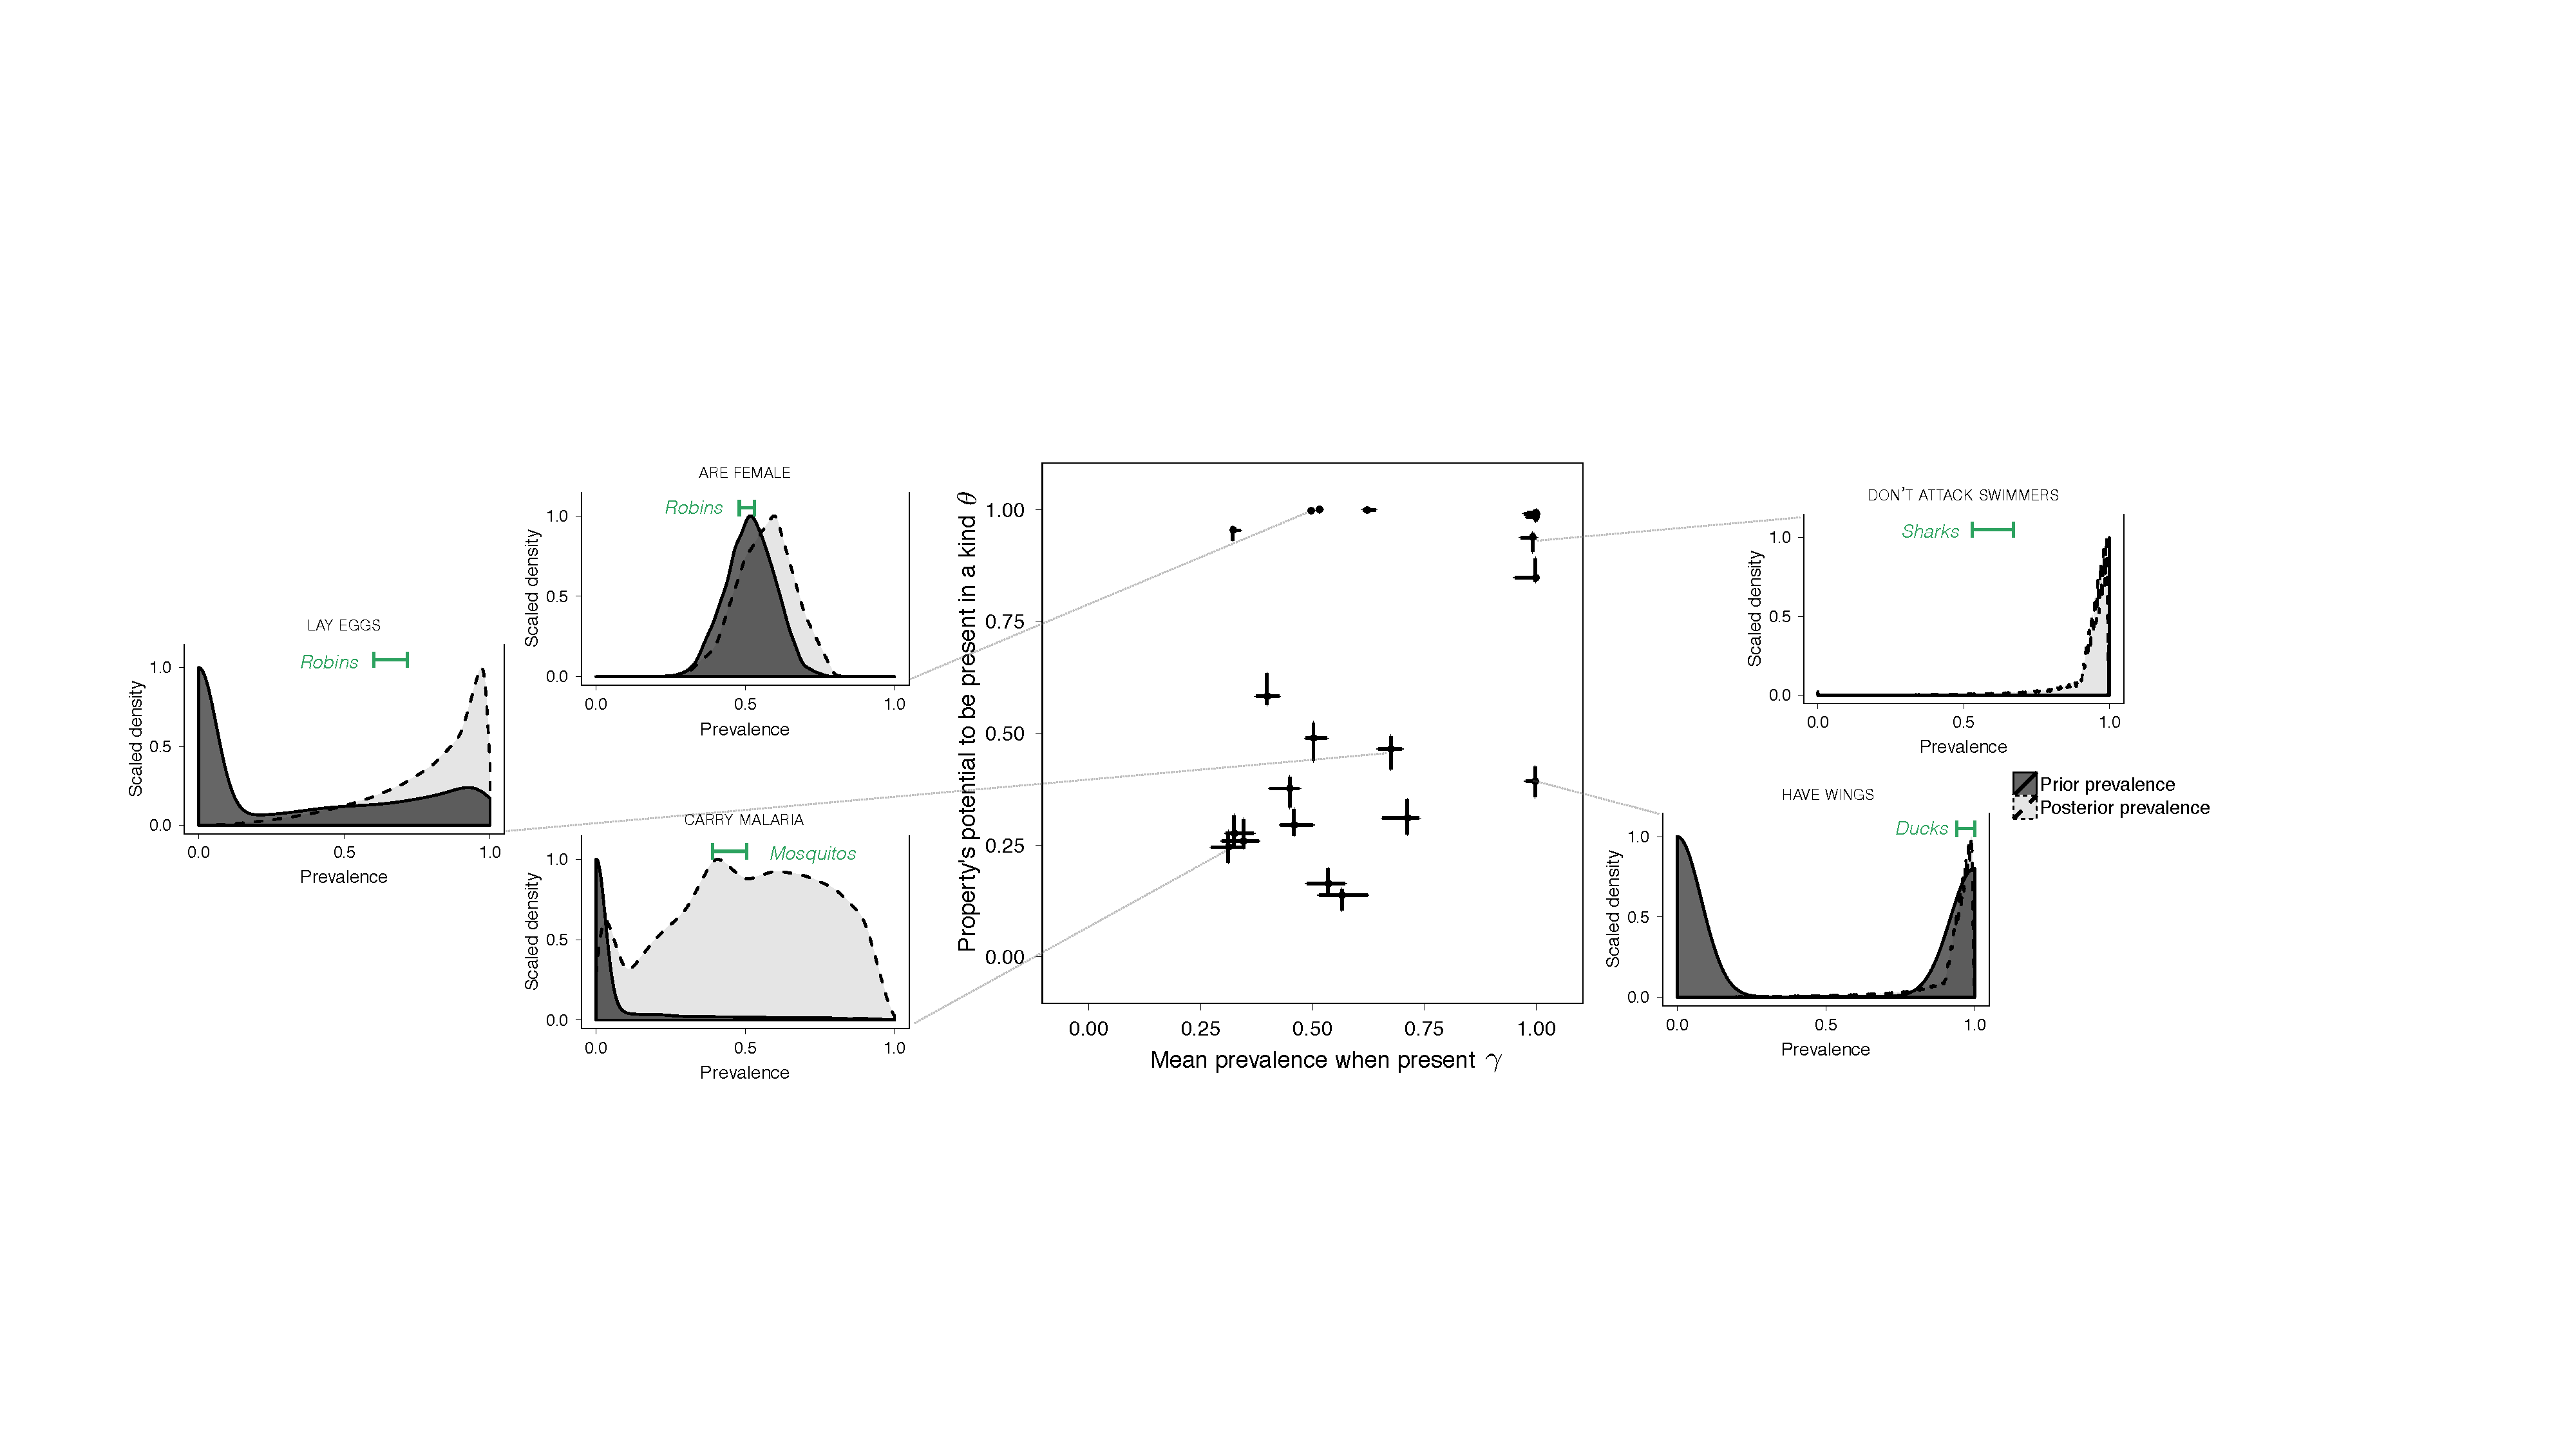
\includegraphics[width=\columnwidth]{generics-priors.pdf}
    \caption{Prevalence prior distributions empirically elicited for twenty-one animal properties.
    Prior distributions are summarized by $\theta$----a property's potential to be present in a category----and $\gamma$----the mean prevalence when it is possible for the property to be present in a category.
    Inset plots display example empirical prior distributions over prevalence together with corresponding $L_1$ model predictions: the posterior after hearing a generic utterance. 
    Intervals on the top of plots show human beliefs about the prevalence of the property within a target category.
    Felicitous generic utterances result when the target prevalence is more likely under the posterior than under the prior.
     Error bars denote 95\% Bayesian credible intervals (same for Figure \ref{fig:prior2}).
    }
  \label{fig:priors1}
\end{figure*}


\subsubsection*{Experiment 1b: Generic endorsements}

 
We tested the degree to which the $S_2$ model, Eq.~\ref{eq:S2}, coupled with the empirically-elicited prevalence priors from Expt.~1a predicted that a given category--property pair (e.g. \textsc{robins} and \textsc{lays eggs}) would result in a felicitous generic (e.g. \emph{Robins lay eggs.}). 
Felicity ratings (n=100) were collected by a two-alternative forced-choice task.

%\subsubsection*{Method}
%
%We recruited 100 participants over MTurk. 
%Participants were shown thirty generic sentences in bare plural form one after another. 
%They were asked to press one of two buttons to signify whether they agreed or disagreed with the sentence. 
%The thirty sentences were presented in a random order between participants and cover a range of conceptual distinctions  \cite{Prasada2013}: characteristic (e.g. \emph{Ducks have wings.}), minority (e.g. \emph{Robins lay eggs.}), striking (e.g. \emph{Mosquitos carry malaria.}), false generalization (e.g. \emph{Robins are female.}), and false (e.g. \emph{Lions lay eggs.}).
%
%\subsubsection*{Analysis and results}
 
From the prevalence-prior data (Expt.~1a), we estimate participants' beliefs about the prevalence of a property \emph{for a given kind} (e.g.~the percentage of \textsc{robins} that \textsc{lay eggs}; see green intervals on Figure \ref{fig:priors1a}).
As a simple baseline hypothesis, we first explore whether these prevalence values themselves predict generic endorsement (e.g.~does the fraction of \textsc{robins} that \textsc{lay eggs} predict the felicity of \emph{Robins lay eggs}?).
A little over half of the variance in truth judgments data is explained by the prevalence of the property within the kind alone (Figure \ref{fig:genericsTJ} left; $r^2 = 0.599$; MSE=0.065). 
This is not surprising given our inclusion of high-prevalence true generics (e.g. \emph{Leopards have spots.}) and low-prevalence false generics (e.g. \emph{Leopards have wings.}). 
However, large deviations remain from an account based purely on target-category prevalence: Generics in which the target category has intermediate prevalence (prevalence quartiles 2 and 3: $ 20\% < prevalence < 64\%$), are not at all explained by prevalence within those categories ($r_{Q2,3}^2 = 0.029$; MSE = 0.110).

The speaker model, $S_2$ in Eq.~\ref{eq:S2}, predicts an endorsement probability for a generic sentence, given prior beliefs for the property and a target prevalence. 
We use the measured within--kind prevalence as the target prevalence that speaker $S_2$ is trying to communicate, and use the
empirically inferred priors from Expt.~1a. The model has one remaining parameter: the speaker optimality parameter $\alpha$ (in Eq.~\ref{eq:S1}).
We integrate out the likely values of this parameter using Bayesian data analytic techniques \cite{LW2014}.
As we see in Figure \ref{fig:genericsTJ} right, the pragmatic speaker model $S_2$, using empirically measured priors, does a very good job of explaining human truth judgments ($r^2=0.981$; MSE=0.003). 
Generics that received definitive agreement or disagreement are predicted to be judged as such by the model (corners of Figure \ref{fig:genericsTJ}), including items for which target-category prevalence is not a good indicator of the acceptability (for prevalence quartiles 2 and 3, $r_{Q2,3}^2=0.955$; MSE=0.005; Figure \ref{fig:genericsTJ}, intermediate shades).
The probabilistic pragmatics model explains the puzzling flexibility of generic truth-conditions as the result of communicative pressures (\emph{be truthful}, \emph{be informative}) operating over diverse prior beliefs about the properties. 



\begin{figure*}
\centering
    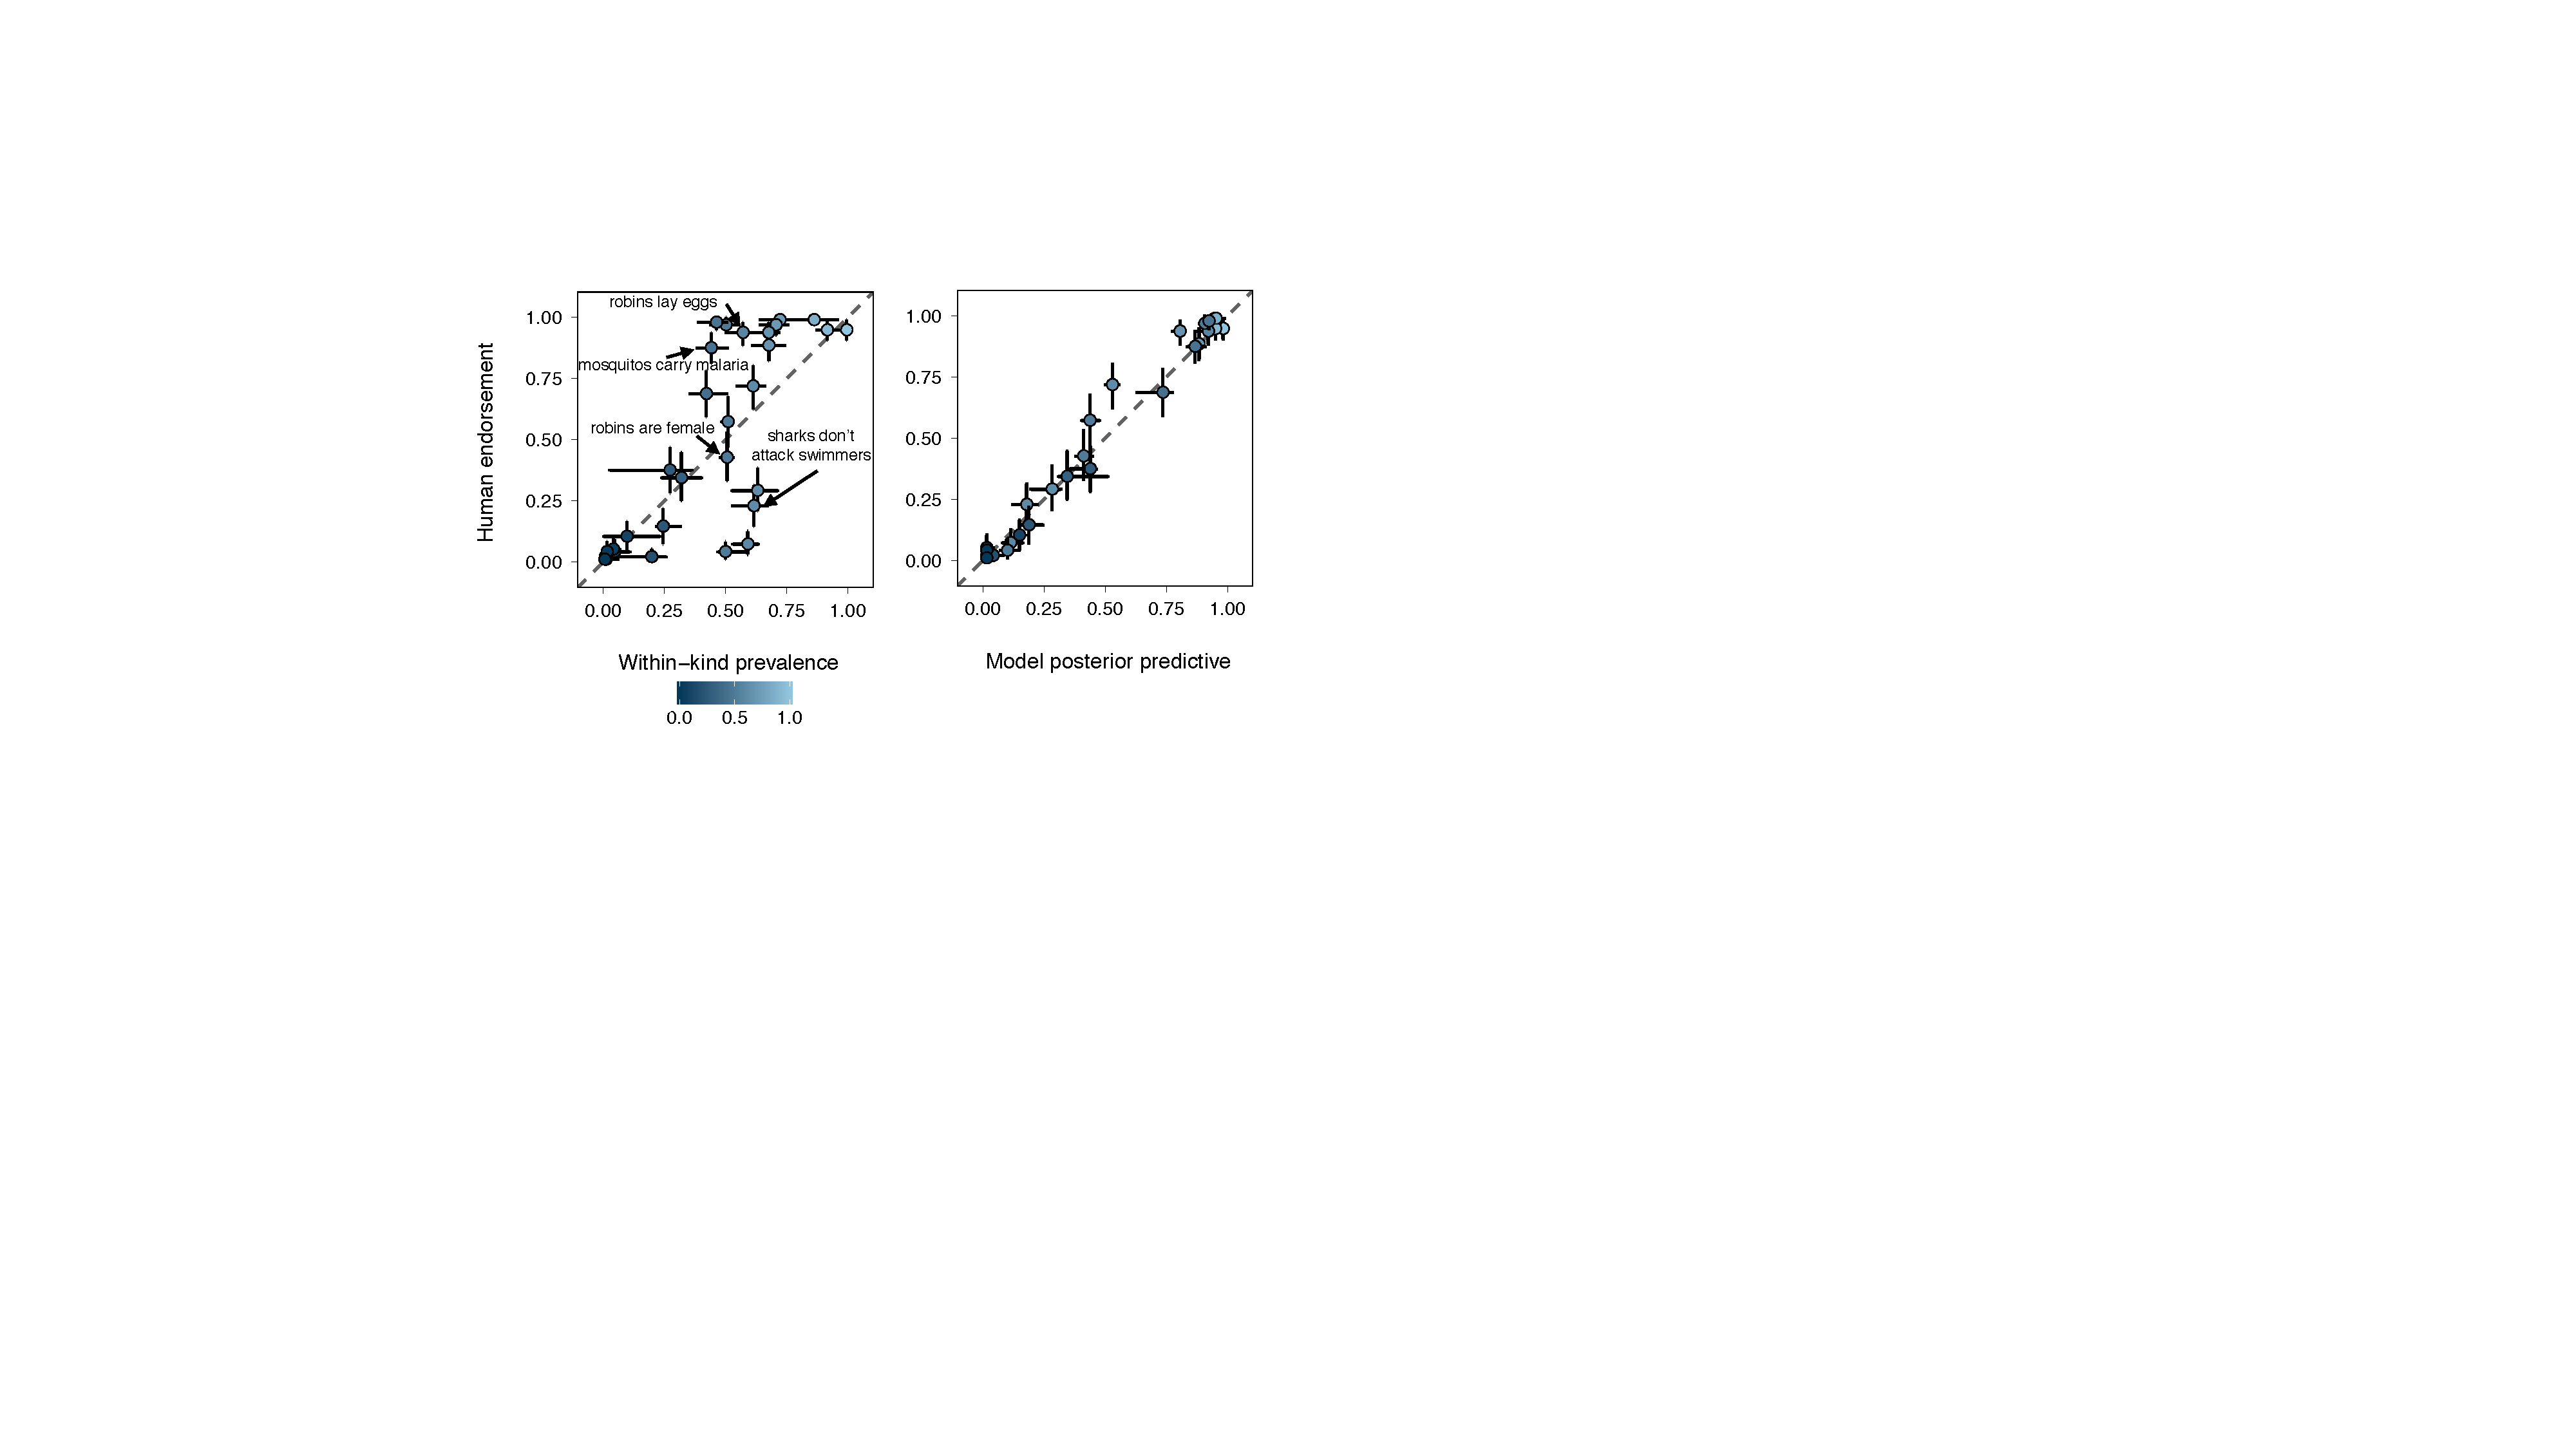
\includegraphics[width=\textwidth]{generics-tj.pdf}
    \caption{Human acceptability judgments and model predictions for thirty generic utterances about familiar animals and properties. 
    Color denotes target-category prevalence of the property, with darker colors indicating lower prevalence. 
    Intermediate prevalences (quartiles 2 \& 3) are in intermediate shades.
    Error bars correspond with 95\% bootstrapped confidence intervals for the participant data and 95\% highest probability intervals for the model predictions.
    }
  \label{fig:genericsTJ}
\end{figure*}




\subsubsection*{Experiment 2a: Prior elicitation for events}

In this experiment we elicit the prior $P(\lambda)$ for different events, so that we can generate model predictions for corresponding habituals.
Given that some individuals rarely or never engage in an event, while others do quite frequently, we would expect the prior to be a mixture distribution between (at least) these two possibilities, similar in spirit to Zero-inflated or Hurdle Models of epidemiological data \cite{hurdleModels}.
Indeed, there may be more than these two possibilities, corresponding to individuals with different traits or demographics (e.g., different expected frequencies depending on age or gender). 

\subsubsection*{Methods}

We recruited 40 participants from Amazon's Mechanical Turk.
Participants were restricted to those with U.S. IP addresses and who had at least a 95\% work approval rating.
The experiment took on average 12 minutes and participants were compensated \$1.25 for their work.

We created thirty-one events organized into pairs or triplets from 5 different conceptual categories: food and drug (e.g. \emph{eats caviar}, \emph{eats peanut butter}), work (e.g. \emph{sells things on eBay}, \emph{sells companies}), clothing (e.g. \emph{wears a suit}, \emph{wears a bra}), entertainment (e.g. \emph{watches professional football}, \emph{watches space launches}) and hobbies (e.g. \emph{runs}, \emph{hikes}). 
Items were chosen to intuitively cover a range of likely frequencies of action, as well as to provide a minimal comparison to another item by having a common superordinate action (e.g. \emph{eating} caviar vs. peanut butter).

For each event, participants were asked two questions, with associated dependent measures:
\begin{enumerate}
\itemsep0em% \{men, women\}
\item ``How many \{men, women\} have \textsc{done action} before?'' \\
Participants responded ``N out of every J.'' by entering a number for N and choosing J from a drop-down menu (options: \{1000 - 10 million\}; default: 1000).
\item ``For a typical \{man, woman\} who has \textsc{done action}  before, how frequently does he or she \textsc{do action}?''\\  
Participants responded ``M times in K.'' by entering a number for M and choosing K from a drop-down menu (options: \{week, month, year, 5 years\}; default: year).
\end{enumerate}
For example, one set of questions read: ``How many men have smoked cigarettes before?''; ``For a typical man who has smoked cigarettes before, how frequently does he smoke cigarettes?''

We anticipated there might be different beliefs about the frequency of events depending on whether the actor is male or female, so we asked about both genders. Participants answered both questions for each gender on each slide (4 questions total per slide, order of male / female randomized between-subjects), and every participant completed all 31 items in random order.
The experiment in full can be viewed at \url{http://stanford.edu/~mtessler/habituals/experiments/priors/priors-2.html}.

\subsection{Data analysis and results}
We built a Bayesian data analysis model for this prior elicitation task.
Question 1 elicits the proportion of people who have done an action before. 
We model this data as coming from a Beta distribution: $d_{1} \sim \text{Beta}(\gamma_{1}, \xi_{1})$. 
Question 2 elicits the rate, or relative frequency, with which a person does the action.
This was modeled by a log-normal distribution: $\ln d_{2} \sim \text{Gaussian}(\mu_{2}, \sigma_{2})$. 
Each item was modeled independently for each gender.
We implemented this model using the probabilistic programming language WebPPL \cite{dippl}, and found the credible values of the parameters by running MCMC for 100,000 iterations, discarding the first 50,000 for burnin.

The priors elicited cover a range of possible parameter values as intended (Figure \ref{fig:priorScatter}, scatter), resulting in parametrized distributions of dramatically different shapes (insets).  
We observe a correlation in our items between the mean \% of Americans who have \textsc{done action} before (Question 1) and the mean log-frequency  of action (Question 2) ($r_{1,2} = 0.74$).
Items that tend to be more popular actions also tend to be more frequent actions (e.g. \emph{wears socks}) and visa-versa (e.g. \emph{steals cars}), though there are notable exceptions (e.g. \emph{plays the banjo} is not popular but done frequently when done at all, as is \emph{smokes cigarettes}; \emph{goes to the movies} is a popular activity though not done very often). 
This diversity is relevant because the speaker model (Eq.~\ref{eq:S2}) will produce habitual sentences (e.g. \emph{Sam goes to the movies vs. the ballet.}) contingent on the shape of the prior distribution. 

From the inferred parameters and assumed functional forms, we get an inferred $P(\lambda)$ modeled as a mixture of individuals with the possibility of carrying out the action and those without the possibility of doing it. 
That is, $P(\lambda)$ was constructed by sampling $\lambda$ as follows:
\begin{align}
\theta & \sim \text{Beta}(\gamma_{1}, \xi_{1}) \nonumber \\ 
\ln \lambda & \sim \begin{cases}
		\text{Gaussian}(\mu_{2}, \sigma_{2}) &\mbox{if } \text{Bernoulli}(\theta) = \textsc{t} \label{eq:priorModel}  \\
				\delta_{\lambda=-\infty} &\mbox{if } \text{Bernoulli}(\theta) = \textsc{f} \\
		\end{cases}
\end{align}
In addition to specifying the correct way to combine our two prior-elicitation questions, using this inferred prior in our language model resolves two technical difficulties: (1) It smooths effects that are clearly results of the response format\footnote{For example, a very common rating is \emph{1 time per year}. Presumably participants would be just as happy reporting \emph{approximately} 1 time per year; the raw data does not reflect this due to demands of the dependent measure.} 
and (2) it better captures the tails of the prior distribution which have relatively little data and need to be regularized by the analysis.
Figure \ref{fig:priorScatter} (right) shows example inferred priors.




\subsubsection*{Experiment 2b: Habitual endorsements}

A present-tense habitual sentence is of the form \textsc{singular noun phrase} $+$ \textsc{present tense simple verb phrase} (e.g. \emph{Bill smokes cigarettes.}).  
We next explore the endorsements of habituals of this form made from the items whose propensity priors were measured in Experiment 1. 

\subsubsection*{Method}


We recruited 150 participants from MTurk. 
The experiment took 4 minutes on average and participants were compensated \$0.55 for their work.

On each trial, participants were presented with a \emph{past frequency statement} for a given event of the form: ``In the past M \{weeks, months, years\}, \textsc{person} \textsc{did x} 3 times''.
For example, \emph{In the past month, Bill smoked cigarettes 3 times}.
The particular intervals used (number M and window \{weeks, months, years\}) were selected after examining the predictions of the speaker model (Eq.~\ref{eq:S2}), for each item independently, to yield a variety of predicted endorsement rates.
The items were the same as in Expt. ~1.

Participants were asked whether they agreed or disagreed with the corresponding habitual sentence: ``\textsc{person does x}'' (e.g. \emph{Bill smokes cigarettes}).
Participants saw 25 out of the 31 items paired randomly with a male or female character name; the other 6 trials were presented with both male and female names (on separate trials; 37 trials total) to explore the nature of the contrast class (see Model section). 
The experiment in full can be viewed at \url{http://stanford.edu/~mtessler/habituals/experiments/truth-judgments/tj-2.html}.

\subsubsection*{Results}
\noindent {\bf Behavioral results}
On each trial of the experiment, the participant was told a person did a particular action 3 times during some time window. 
Figure \ref{fig:tjScatters} (left) shows the correspondence between the frequency of the event (normalizing to a 5-year time scale and taking the logarithm) and the felicity of the corresponding habitual sentence. 
It is clear that a habitual sentence can receive strong agreement even when the actions are very infrequent (log frequency $\sim$ 1; 3 times in a 5-year interval; e.g. \emph{writes novels}, \emph{steals cars}).
We also see even when actions are done relatively frequently (e.g. 3 times in a one month interval; log frequency $\sim$ 5), there are habitual sentences participants are reluctant to endorse completely (e.g. \emph{wears socks}, \emph{drinks coffee}). 
In our data, actions completed with a high frequency (3 times in a one week interval; log frequency $\sim$ 6.5) receive at least 75\% endorsement, though there is still variability among them (e.g. between 10-25\% of people disagree with \emph{wears a watch} and \emph{wears a bra}). %, suggesting that even actions that are completed almost everyday can insufficient to generalize.
Overall, frequency of action predicts only a fraction of the variability in responses ($r^2(93) = 0.33$).
For actions that are done on the time scale of years or longer (lower median of frequency), frequency itself no longer explains the endorsements ($r^2(50) = 0.07$)

We further examined the six items for which we observed gender differences in the prior elicitation task (Expt.~1).
We find no differences between endorsements of the habitual of characters with male and female names, and overall, the mean endorsements by gender are strongly correlated $r(93) = 0.91$. 
This may be because the felicity of habitual sentences depends on a comparison to individuals of both genders (i.e, the \emph{contrast class} is other people; not just other men or women). 
Less interestingly, the lack of a difference may be the result of gender being not very salient in our paradigm, perhaps because the names used were not sufficiently gendered.

\subsubsection*{Discussion}

We presented a formal model for the evaluation of statements that communicate generalizations.
The model decides if a generic sentence is a pragmatically useful way to describe a category taking into account the listener's prior beliefs about the property---how common it is and the likely prevalence (measured in Expt.~1a, 2a).
We validated this model by eliciting felicity judgments for generic and habitual sentences covering diverse properties and activities (Expt.~1b, 2b).
To our knowledge, the experiments presented here are first empirical investigations into the truth conditions of habitual sentences and the first test of a formal model of habitual language.



%Yet the meaning of generic language is philosophically puzzling and has resisted precise formalization.
%We explore the idea that the core meaning of a generic sentence is simple but underspecified, 
%and that general principles of pragmatic reasoning are responsible for establishing the precise meaning in context.
%Building on recent probabilistic models of language understanding, we provide a formal model for the evaluation and comprehension of generic sentences. 
%This theory provides the mathematical bridge between the words we use and the concepts they describe.


\bibliographystyle{apacite}

\setlength{\bibleftmargin}{.125in}
\setlength{\bibindent}{-\bibleftmargin}

\bibliography{generics-spp}

\end{document}

